\documentclass[11pt]{article}
\usepackage[utf8]{inputenc}
\usepackage{amsmath}
\usepackage{amsfonts}
\usepackage{amssymb}
\usepackage{bbm}
\usepackage{vmargin}
\usepackage{bm}
\usepackage{nicefrac}
\usepackage{cleveref}
\usepackage{float}
\usepackage{cancel}

\setmargins{2cm}       % margen izquierdo
{1.5cm}                % margen superior
{16cm}                 % anchura del texto
{23cm}                 % altura del texto
{10pt}                 % altura de los encabezados
{1cm}                  % espacio entre el texto y los encabezados
{1.5cm}                % altura del pie de página
{1cm}                  % espacio entre el texto y el pie de página

%El paquete relsize y bbm es para escribir la indicadora
\usepackage{relsize}
\usepackage{bbm}

\usepackage{xeboiboites}

\newboxedtheorem[
	small box style={
		fill=violet!20,
		draw=violet,
		%decoration={penciline},
		decorate},
    big box style={
    		fill=violet!10,
    		draw=violet,
        %decoration={penciline},
        decorate},
    headfont=\bfseries]%
{IrvingBox}{}{}

%Manera de escribir la indicadora:
%\indicadora{(0,\infty)}{(x)}
\newcommand{\indicadora}[2]{\mathlarger{\mathbbm{1}}\,_{#1}#2}

\newcommand\independent{\protect\mathpalette{\protect\independenT}{\perp}}
\def\independenT#1#2{\mathrel{\rlap{$#1#2$}\mkern2mu{#1#2}}}

\def\X{\mathbf{X}}
\def\Y{\mathbf{Y}}
\def\Z{\mathbf{Z}}

\def\x{\mathbf{x}}
\def\y{\mathbf{y}}
\def\z{\mathbf{z}}

\def\P{\mathbb{P}}
\def\V{\mathbb{V}}
\def\E{\mathbb{E}}

\def\R{\mathbb{R}}
\def\N{\mathbb{N}}

\def\Normal{\mathcal{N}}

\def\sample{\mathcal{D}_n}

\def\Ymis{Y_{\text{mis}}}
\def\Yobs{Y_{\text{obs}}}
\def\Ycomp{Y_{\text{comp}}}

\newcommand{\anguls}[1]{\left\langle #1 \right\rangle}      %   <>
\newcommand{\llavs}[1]{\left\lbrace #1 \right\rbrace}       %   {}
\newcommand{\corchet}[1]{\left\lbrack #1 \right\rbrack}     %   []
\newcommand{\parent}[1]{\left( #1 \right)}                  %   ()
\newcommand{\abs}[1]{\lvert#1\rvert}                        %   ||
\newcommand{\norm}[1]{\lVert#1\rVert}                       %   || ||

\DeclareMathOperator*{\argmin}{arg\,min}
\DeclareMathOperator*{\argmax}{arg\,max}
\DeclareMathOperator*{\minimize}{\text{minimize}}
\DeclareMathOperator*{\maximize}{\text{maximize}}
\DeclareMathOperator*{\sign}{\text{sign}}

\begin{document}
\title{Finding optimum price to maximize the expected gain}
\author{Irving Gómez Méndez}
\date{}
\maketitle

\section{Creating the model}

Assume we have the unitary cost, unitary price, and the amount of products sold, $C,P,Q$.

According to the law of demand, the more expensive the product is, the less it is sold, which can be expressed in the next mathematical model:
\[Q=\beta_0-\beta_1 P+\varepsilon,\quad \beta_0,\beta_1>0,\,\varepsilon\sim\Normal(0,\sigma^2).\]
Or, equivalently,
\[Q\sim\Normal\Big(\beta_0-\beta_1 P, \sigma^2\Big).\]
Let be $U$ the gain, it can be expressed as
\begin{align*}
U &= Q(P-C) \\\\
&= (\beta_0-\beta_1 P+\varepsilon)(P-C) \\\\
& = \underbrace{(\beta_0-\beta_1 P)(P-C)}_{\mu_U}+(P-C)\varepsilon.
\end{align*}
Or, equivalently,
\[U\sim\Normal\Big(\mu_U,(P-C)^2\sigma^2\Big)\]
Note that
\[\mu_U=-\beta_0C+(\beta_0+\beta_1C)P-\beta_1P^2.\]
We can find $P^\star$ that maximizes the expected gain, $\mu_U$.
\[\frac{\partial \mu_U}{\partial P}=\beta_0-\beta_1C-2\beta_1 P\]
\[\left.\frac{\partial \mu_U}{\partial P}\right|_{P=P^\star}=0.\]
Thus,
\begin{IrvingBox}[$P^\star,Q^\star,U^\star$]
\vspace{-0.5cm}
\begin{align*}
P^\star &= \frac{\beta_0+\beta_1C}{2\beta_1} \\\\
Q^\star &= \beta_0-\beta_1P^\star+\varepsilon \\\\
U^\star &= Q^\star(P^\star-C)
\end{align*}
\end{IrvingBox}

\section{Fitting the model}

For instance, assume that we count with the next data:
\begin{center}
\begin{tabular}{|c|c|c|c|c|c|c|c|c|c|c|c|c|c|c|c|}
\hline 
Price & 21 & 19 & 20 & 15 & 18 & 18 & 7 & 16 & 14 & 9 & 11 & 13 & 10 & 10 & 10 \\ 
\hline 
Quantity & 3 & 3 & 7 & 6 & 10 & 15 & 16 & 13 & 9 & 15 & 9 & 15 & 12 & 18 & 21 \\ 
\hline 
\end{tabular}
\end{center}
With a constant cost $C=3$.

With the next scatter plot between the price and the quantity sold.
\begin{center}
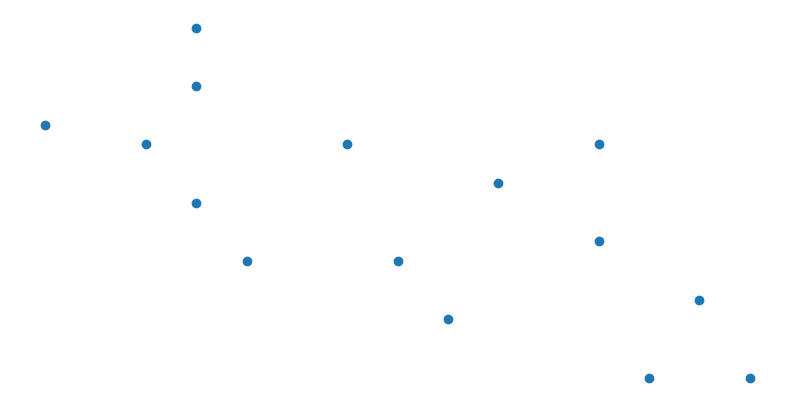
\includegraphics[width=0.75\textwidth]{Images/PriceQuantityScatterplot}
\end{center}

Thus, our model can be represented by the next probabilistic graphical model:
\begin{center}
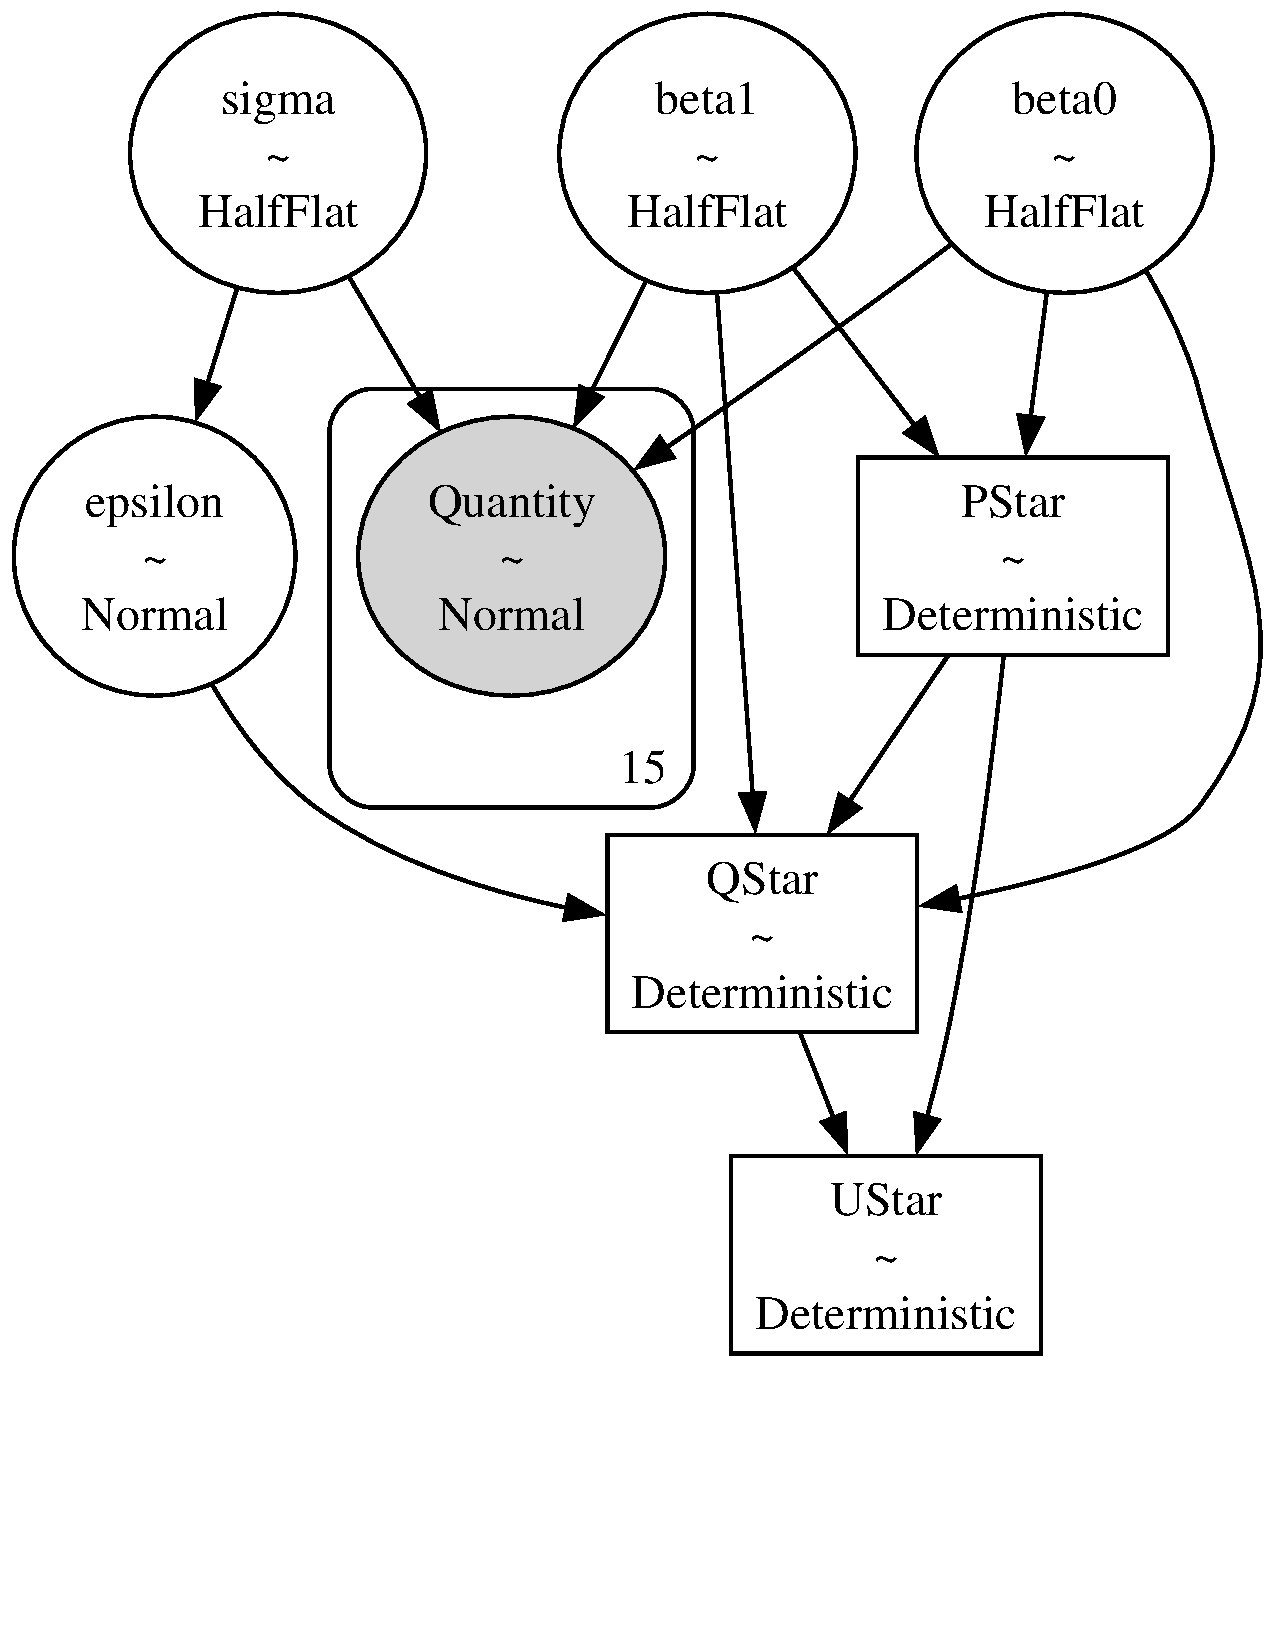
\includegraphics[width=0.5\textwidth]{Images/MaximizingGainModel}
\end{center}
\vspace{-1.5cm}
Once the model has been fitted, we get the next posterior distributions for $P^\star,Q^\star,U^\star$
\begin{center}
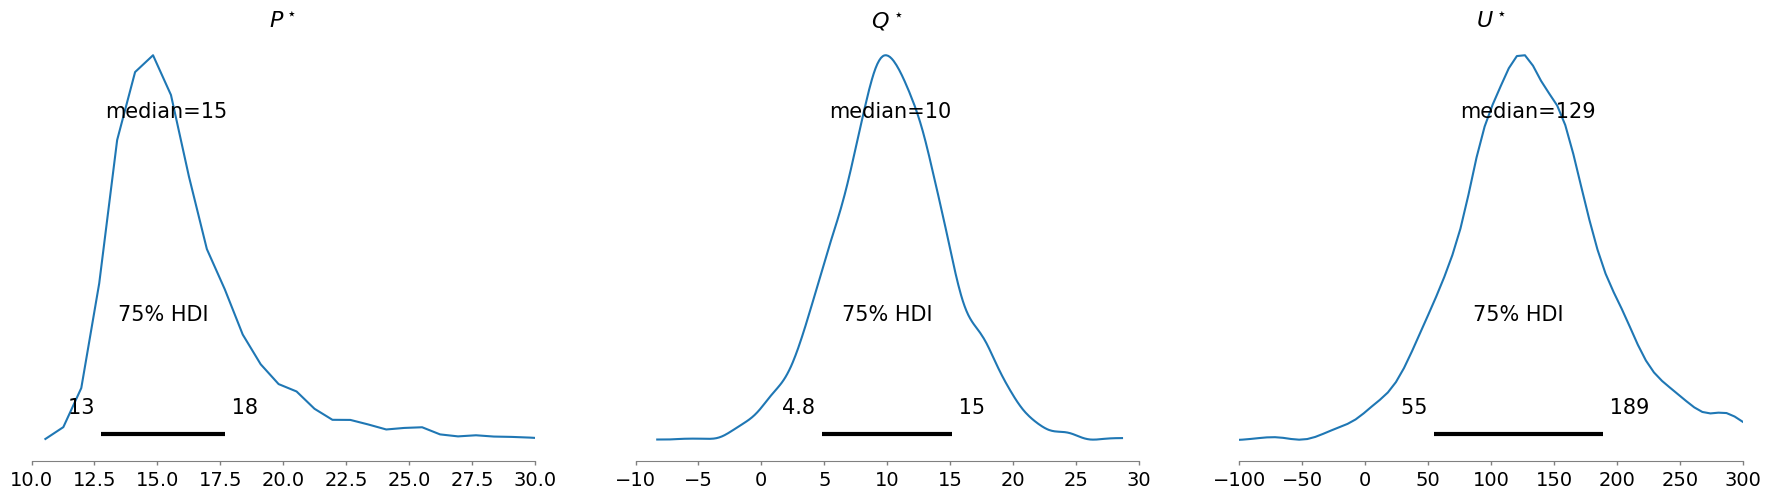
\includegraphics[width=\textwidth]{Images/OptimumQuantities}
\end{center}

\section{Confidence and prediction intervals}

On the other hand, using
\begin{align*}
Q \sim \Normal\Big(\mu_Q, \sigma^2\Big), \quad &\mu_Q=\beta_0-\beta_1 P, \\\\
U \sim\Normal\Big(\mu_U,(P-C)^2\sigma^2\Big), \quad &\mu_U=-\beta_0C+(\beta_0+\beta_1C)P-\beta_1P^2,
\end{align*}
we can create posterior confidence bands for $\mu_Q$ and $\mu_U$, and posterior prediction bands for $Q$ and $U$.

Taking all these statistics into account, we can represent our results in the next plots, showing the relationship between the price and the quantity sold, and the price and the gain.
\begin{center}
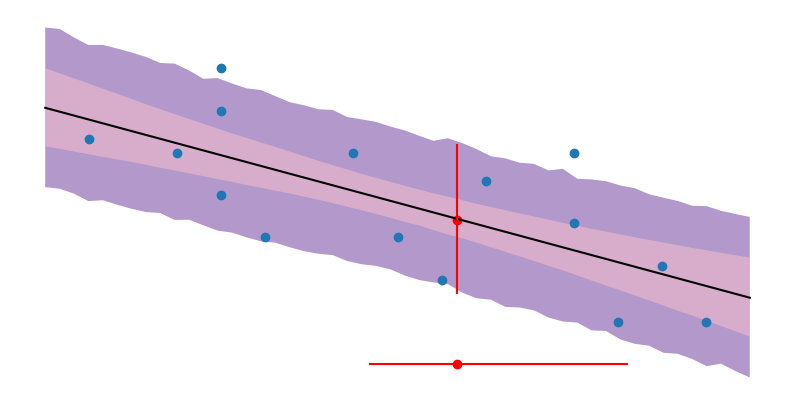
\includegraphics[width=0.66\textwidth]{Images/PriceQuantityRegression}
\end{center}
\begin{center}
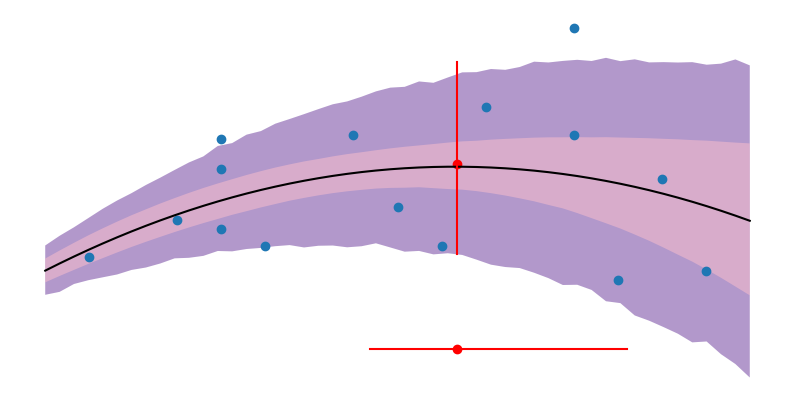
\includegraphics[width=0.66\textwidth]{Images/PriceGainRegression}
\end{center}

\end{document}